\Exhibit{OpenSourceWikipedia}{%
    Статья в Wikipedia про `open source'
}

Это скриншот страницы Wikipedia про `open source'.
Здесь сказано:

\ParagraphQuote{%
    Многие крупные формальные организации были созданы для поддержки развития
    движения open-source, включая Apache Software Foundation,
    которая поддерживает проекты, такие как фреймворк Apache Hadoop и HTTP-сервер Apache HTTP.%
}

\begin{center}
    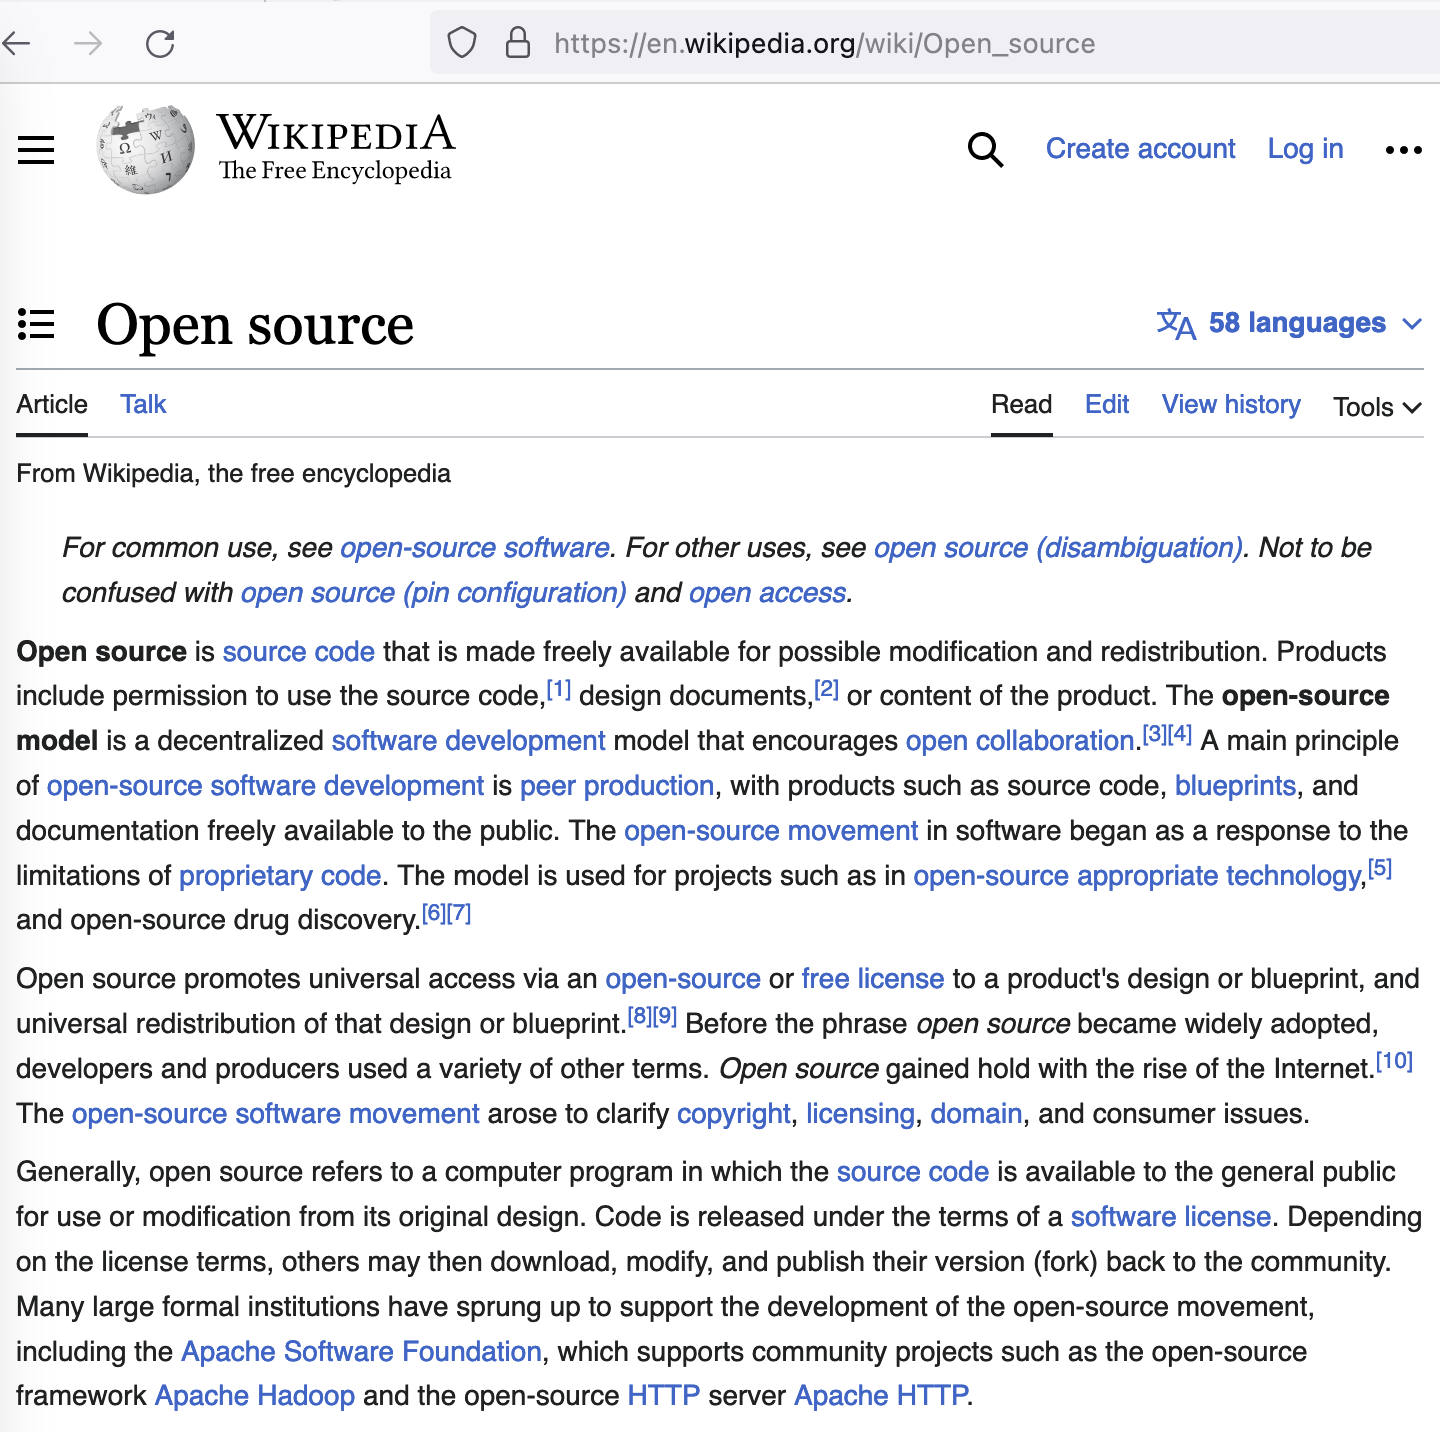
\includegraphics[width=35em]{open-source-wikipedia}
\end{center}

\pagebreak
